\documentclass{beamer} 

\mode<presentation>
{
  \usetheme{Berkeley}
  % or ...

  \setbeamercovered{transparent}
  % or whatever (possibly just delete it)
}

\usepackage{tikz}
\usepackage{graphicx}
\usepackage[english]{babel}


\usepackage[utf8]{inputenc}
% or whatever

\usepackage{times}
\usepackage[T1]{fontenc}
% Or whatever. Note that the encoding and the font should match. If T1
% does not look nice, try deleting the line with the fontenc.


\title[Power and Multiple Hypothesis Testing] % (optional, use only with long paper titles)
{Power and Multiple Hypothesis Testing}

\subtitle
{}

\author[Christensen] % (optional, use only with lots of authors)
{Garret~Christensen\inst{1}}
% - Give the names in the same order as the appear in the paper.
% - Use the \inst{?} command only if the authors have different
%   affiliation.

\institute[Universities of Somewhere and Elsewhere] % (optional, but mostly needed)
{
  \inst{1}%
  UC Berkeley:\\
  Berkeley Initiative for Transparency in the Social Sciences\\
  Berkeley Institute for Data Science\\
  }
% - Use the \inst command only if there are several affiliations.
% - Keep it simple, no one is interested in your street address.

\date[BITSS2014] % (optional, should be abbreviation of conference name)
{IDB, March 2018\\
Slides available online at \url{http://www.github.com/BITSS/IDBMarch2018}}
% - Either use conference name or its abbreviation.
% - Not really informative to the audience, more for people (including
%   yourself) who are reading the slides online

\subject{Research Transparency}
% This is only inserted into the PDF information catalog. Can be left
% out. 

\pgfdeclareimage[height=2cm]{university-logo}{../Images/BITSSlogo.png}
\logo{\pgfuseimage{university-logo}}

% If you have a file called "university-logo-filename.xxx", where xxx
% is a graphic format that can be processed by latex or pdflatex,
% resp., then you can add a logo as follows:

% \pgfdeclareimage[height=0.5cm]{university-logo}{university-logo-filename}
% \logo{\pgfuseimage{university-logo}}



% Delete this, if you do not want the table of contents to pop up at
% the beginning of each subsection:
%\AtBeginSubsection[]
%{
%  \begin{frame}<beamer>{Outline}
%    \tableofcontents[currentsection,currentsubsection]
%  \end{frame}
%}


% If you wish to uncover everything in a step-wise fashion, uncomment
% the following command: 

\beamerdefaultoverlayspecification{<.->}


\begin{document}

\begin{frame}
  \titlepage
\end{frame}




% Structuring a talk is a difficult task and the following structure
% may not be suitable. Here are some rules that apply for this
% solution: 

% - Exactly two or three sections (other than the summary).
% - At *most* three subsections per section.
% - Talk about 30s to 2min per frame. So there should be between about
%   15 and 30 frames, all told.

% - A conference audience is likely to know very little of what you
%   are going to talk about. So *simplify*!
% - In a 20min talk, getting the main ideas across is hard
%   enough. Leave out details, even if it means being less precise than
%   you think necessary.
% - If you omit details that are vital to the proof/implementation,
%   just say so once. Everybody will be happy with that.
%%%%%%%%%%%%%%%%%%%%%%%%%%%%%%%%%%%%%%%%%%%%%%%%%%%%%%%%%%%%%%%%%%%%%%%
%%%%%%%%%%%%%%%%%%%%%%%%%%%%%%%%%%%%%%%%%%%%%%%%%%%%%%%%%%%%%%%%%%%%%
\begin{frame}{Outline}
  \tableofcontents
  % You might wish to add the option [pausesections]
\end{frame}

\section {Introduction}
{ % all template changes are local to this group.
    \setbeamertemplate{navigation symbols}{}
    \begin{frame}[plain]
        \begin{tikzpicture}[remember picture,overlay]
            \node[at=(current page.center)] {
                \href{https://www.bitss.org/}{\includegraphics[width=\paperwidth]{../Images/bitsslogo.png}}
            };
        \end{tikzpicture}
     \end{frame}
}

\begin{frame}{What is Statistical Power?}
The power of a statistical hypothesis test is the probability that the test correctly rejects the null hypothesis when it is false.
\vskip0.25in
That is, if there's a real effect, what's the likelihood you'll detect it? 80\% is the standard.
\end{frame}

\begin{frame}{What is Statistical Power?}
In terms of Type I (false positive) and Type II (false negative) errors: 
\begin{itemize}
\item Type I error rate is $\alpha$
\item Type II error rate is $\beta$
\item Power is $1-\beta$.
\end{itemize}
 \end{frame}

\begin{frame}{$Power=1-\beta$}
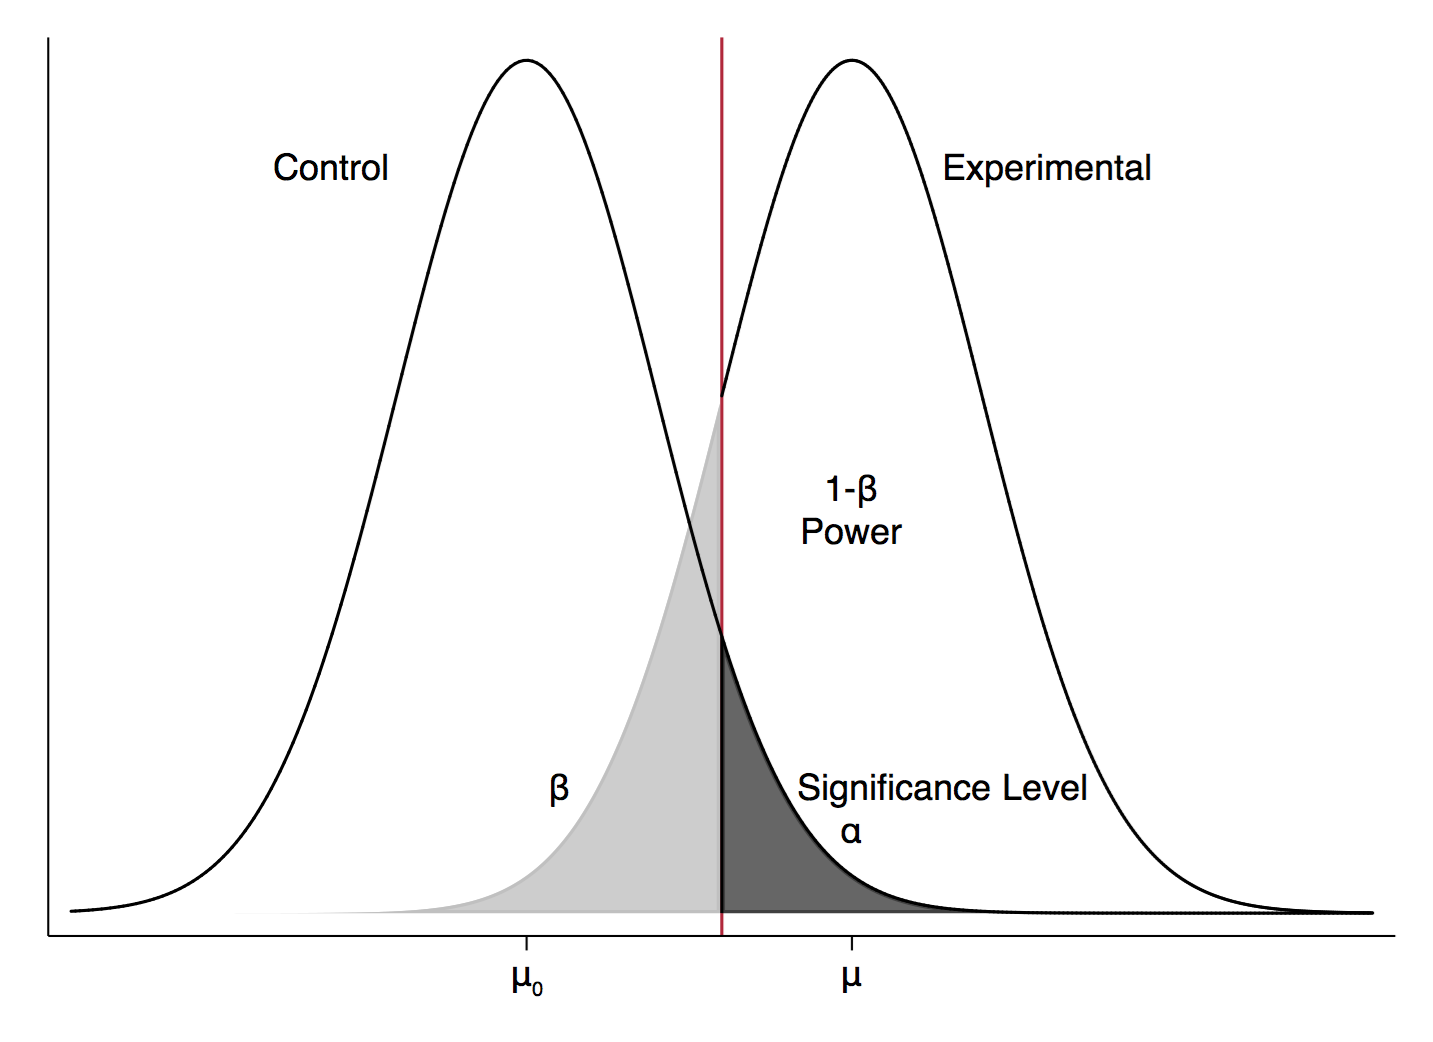
\includegraphics[height=3in]{../Images/powerfig1.png}
\end{frame}

\begin{frame}{Less noise, more power}
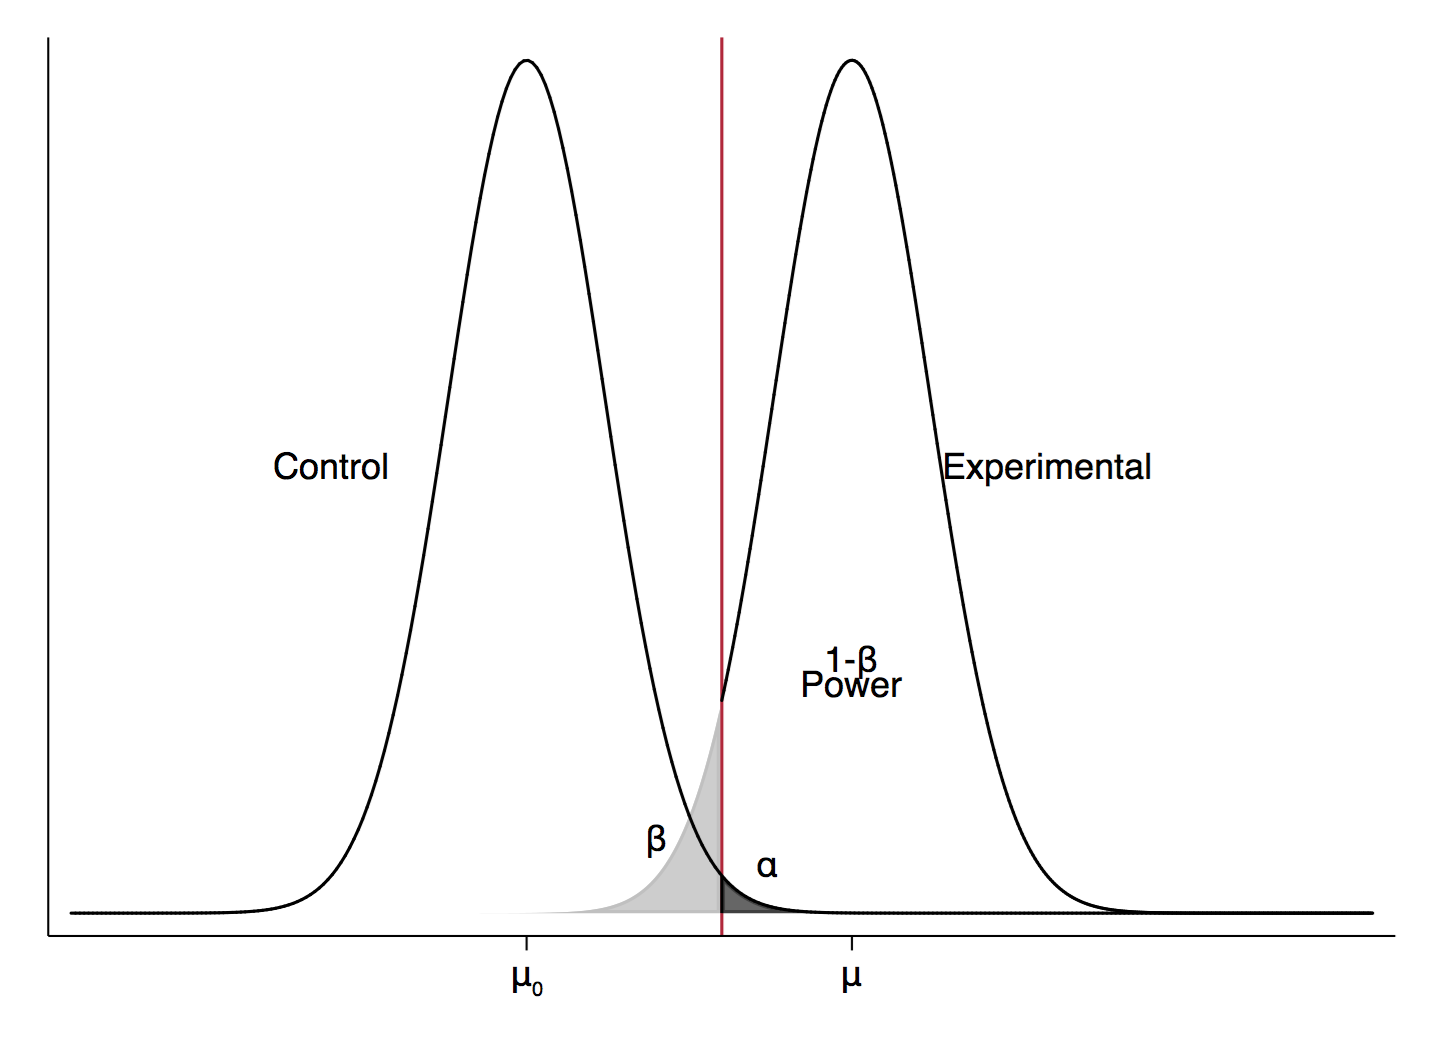
\includegraphics[height=3in]{../Images/powerfig2.png}
\end{frame}

\begin{frame}{Larger true effect, more power}
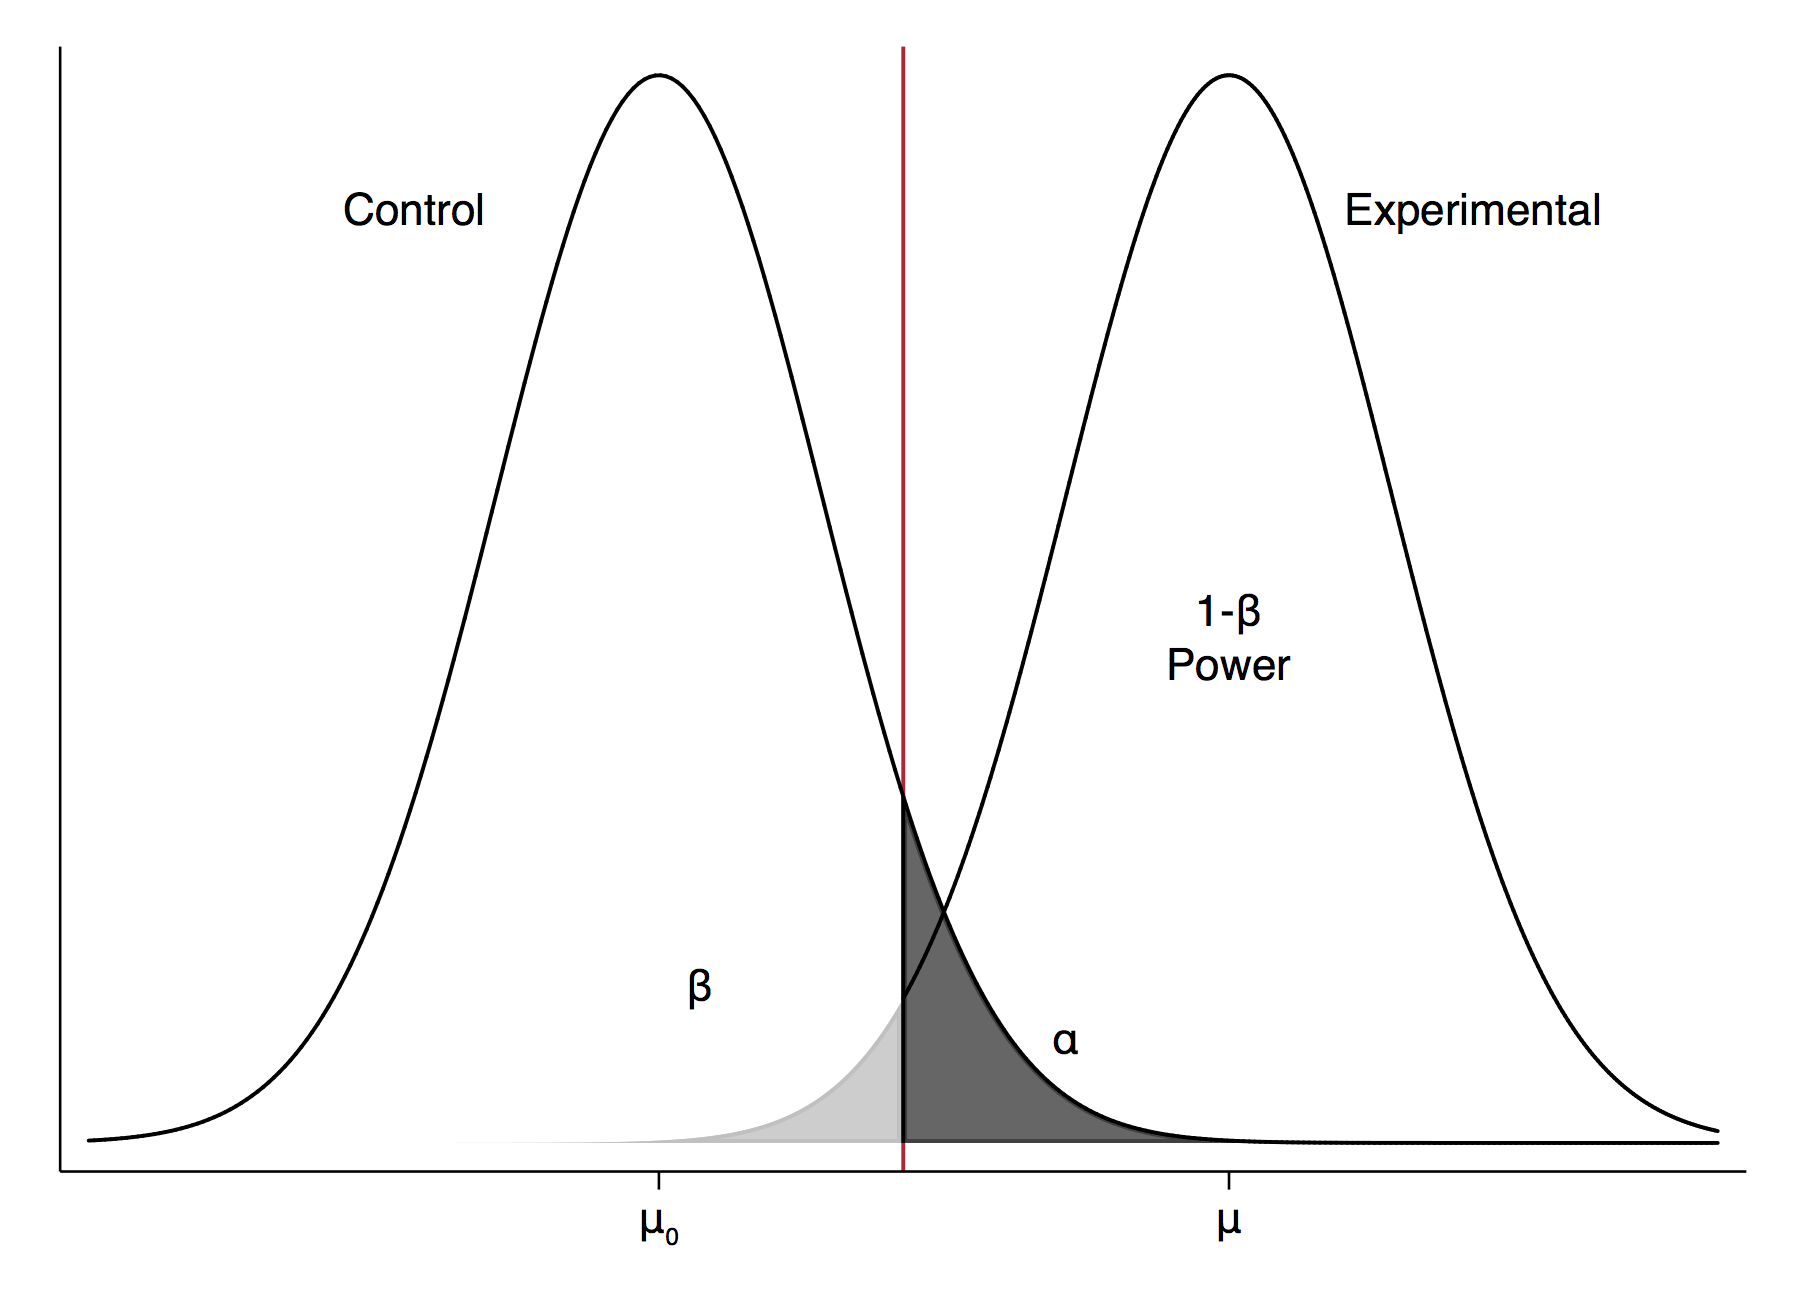
\includegraphics[height=3in]{../Images/powerfig3.png}
\end{frame}


\begin{frame}{Derivation}
\[Power = 1 - \beta = Pr(\overset{\overline{}}{Y} \geq \ \mu_{0} + z_{1 - \alpha}\sigma/\sqrt{}n|H_{1}:\ \mu > \mu_{0})\]

\[= 1 - Pr(\overset{\overline{}}{Y} < \ \mu_{0} + z_{1 - \alpha}\sigma/\sqrt{}n|H_{1})\]

\[= 1 - Pr(\frac{\overset{\overline{}}{Y} - \mu}{\frac{\sigma}{\sqrt{n}}} < \ \frac{\mu_{0} + \frac{z_{1 - \alpha}\sigma}{\sqrt{n}} - \mu}{\frac{\sigma}{\sqrt{n}}}|H_{1})\]

\[= 1 - Pr(\frac{\overset{\overline{}}{Y} - \mu}{\frac{\sigma}{\sqrt{n}}} < \ \frac{\mu_{0} - \mu}{\frac{\sigma}{\sqrt{n}}} + z_{1 - \alpha}|H_{1})\]

\[= 1 - \Phi(\ \frac{\mu_{0} - \mu}{\frac{\sigma}{\sqrt{n}}} + z_{1 - \alpha}|H_{1})\]

\[= \Phi(\ \frac{\mu_{0} - \mu}{\frac{\sigma}{\sqrt{n}}} - z_{1 - \alpha}|H_{1})\]
\end{frame}

\begin{frame}{Increasing Power}
\[= \Phi(\ \frac{\mu_{0} - \mu}{\frac{\sigma}{\sqrt{n}}} - z_{1 - \alpha}|H_{1})\]

Hopefully the equation makes clear that:
\begin{itemize}
\item larger $n$
\item lower $\sigma$
\item larger true effect size $(\mu_0-\mu)$
\item and a larger $\alpha$, though that's kind of cheating
\end{itemize}
 all increase power.
\end{frame}

\begin{frame}{Rearranging}
Rather than solving for power, you may want to solve for the minimum detectable effect (MDE). 

\[MDE = \left( t_{\beta} + t_{\alpha} \right)*\sqrt{\frac{1}{P(1 - P)}}\sqrt{\frac{\sigma^{2}}{n}}\]

Or, if you've got unlimited funds, pick the minimum biologically or practically meaningful effect, (or your estimate from previous literature of how big the effect will be) and solve for $n$.
\end{frame}

\begin{frame}{Design Effect}
We've so far assumed independent observations, which isn't the case if we cluster treatment. Multiply MDE by the Design Effect:

$$\sqrt{1+(n-1)\rho}$$

Where $n$ is households per sampling unit, and $\rho$ is the intracluster correlation--variance between clusters divided by sum of within and between.
\end{frame}

\begin{frame}{Complications}
Clusters not equal sized? Use the coefficient of variation, but it may not matter much. \href{https://doi.org/10.1093/ije/dyl129}{(Eldridge, Ashby, Kerry 2006)}
\vskip0.25in
You get the most power with equal proportions of treated/control. If treatment is very expensive, maximize power subject to your budget constraint. \href{http://www.sciencedirect.com/science/article/pii/S1573447107040612}{(Randomization Toolkit: Duflo, Glennerster, and Kremer 2007)}
\vskip0.25in
Panel with serial correlation? \href{https://static1.squarespace.com/static/558eff8ce4b023b6b855320a/t/59e932358dd041e0d712fff8/1508454965886/BPW\_Power\_Calculations\_2017\_10\_19.pdf}{(Burlig, Preonas, Woerman 2017)}
\vskip0.25in
Complicated? Just simulate it. \href{https://doi.org/10.1186/1471-2288-11-94}{(Arnold et al. 2011)}
\end{frame}

\section{Problems in Econ}
\begin{frame}{Problem of Low Power}
So what happens if we have low power?
\begin{itemize}
\item
More false negatives (Type II error, just $\beta$).
\item
More false positives! More precisely, the likelihood that a reported effect represents a true finding decreases.
\end{itemize}
\end{frame}

\begin{frame}[label=Ioannidis]{Ioannidis 2005}
\href{http://journals.plos.org/plosmedicine/article?id=10.1371/journal.pmed.0020124}{``Why most published research findings are false'' (Ioannidis 2005)}, cited 5600 times.

\[PPV = Pr(True|T > t_{\alpha})\]


\[= \frac{(1 - \beta) \cdot R}{(1 - \beta)R + \alpha}\]

\begin{itemize}
\item
  R is ratio of true relationships to non-relationships tested in a literature.
\end{itemize}

\hyperlink{derive}{\beamerbutton{Derivation}}
\end{frame}

\begin{frame}{How Common in Economics?}
Quite
\end{frame}

{ % all template changes are local to this group.
    \setbeamertemplate{navigation symbols}{}
    \begin{frame}[plain]q
        \begin{tikzpicture}[remember picture,overlay]
            \node[at=(current page.center)] {
                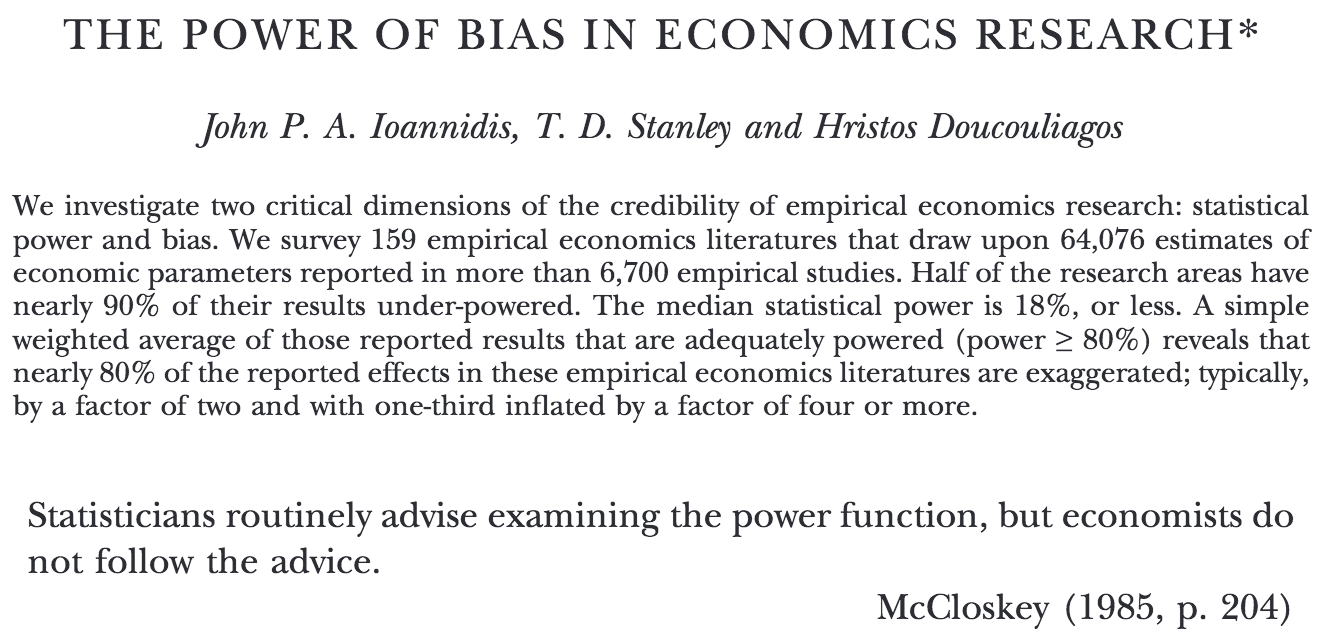
\includegraphics[width=\paperwidth]{../Images/Stanley2017.png}
            };
        \end{tikzpicture}
     \end{frame}
}

\begin{frame}{Ioannidis, Stanley, Doucouliagos 2017}
\begin{quote}If we adopt the conventional 5\% level of statistical significance and 80\% power
level, as well, then the `true effect' will need to be 2.8 standard errors from zero to
discriminate it from zero. The value of 2.8 is the sum of the usual 1.96 for a
significance level of 5\% and 0.84 that is the standard normal value that makes a 20/80\% split in its cumulative distribution. Hence, for a study to have adequate power, its
standard error needs to be smaller than the absolute value of the underlying effect
divided by 2.8. We make use of this relationship to survey adequate power in
economics.
\end{quote}
\end{frame}
%%%%%%%%%%%%%%%%%%%%%%%%%%%%%%%%%%%%%%%%%%%%%%%%%%%%%%%%%%%%%%%%%%%%%%%%%%

\begin{frame}
\begin{center}
Questions?
\vspace{1in}


\Huge{Thank you!}
\end{center}
\end{frame}

\begin{frame}[label=derive]{Derivation of PPV I}
\[PPV = Pr(True|T > t_{\alpha})\]

Prior to the study, the quantities involved are as follows:

\begin{itemize}
\item
  Probability of a relationship being true: \(\frac{R}{R + 1}\)
\item
  Probability of a relationship being false:
  \(1 - \frac{R}{R + 1} = \frac{1}{R + 1}\)
\item
  Probability of finding a positive statistical association given that
  the relationship is false: \(\alpha\)
\item
  Probability of finding a positive statistical association given that
  the relationship is true (i.e., power): \(1 - \beta\)
\end{itemize}
\end{frame}

\begin{frame}[label=derive]{Derivation of PPV II}
Bayes' law says that \(Pr(A|B) = \frac{Pr(B|A)Pr(A)}{Pr(B)}\) , though
it is almost always the case that the denominator is more useful when
written out with the law of total probability, as follows:

\(Pr(A|B) = \frac{Pr(B|A)Pr(A)}{Pr(B|A)Pr(A) + Pr(B|\neg A)Pr(\neg A)}\).

By using Bayes' law, we know that:
\tiny{
\[Pr(True|T > t_{\alpha}) = \frac{Pr(T > t_{\alpha}|True) \cdot Pr(True)}{Pr(T > t_{\alpha}|True) \cdot Pr(True) + Pr(T > t_{\alpha}|False \cdot Pr\left( \text{False} \right))}\]}
\end{frame}

\begin{frame}[label=derive]{Derivation of PPV III}
Substituting, we find:

\[Pr(True|T > t_{\alpha}) = \frac{(1 - \beta)\frac{R}{R + 1}}{(1 - \beta)\frac{R}{R + 1} + \alpha \cdot \frac{1}{R + 1}}\]

\[Pr(True|T > t_{\alpha}) = \frac{\frac{(1 - \beta) \cdot R}{R + 1}}{\frac{(1 - \beta)R + \alpha}{R + 1}}\]

Simplifying:

\[Pr(True|T > t_{\alpha}) = \frac{(1 - \beta) \cdot R}{(1 - \beta)R + \alpha} = \frac{(1 - \beta)R}{R - \beta R + \alpha}\]

This is the same as the formula in Ioannidis (2005) and equation 1
above.
\hyperlink{Ioannidis}{\beamergotobutton{Back}}
\end{frame}


\end{document}

